\documentclass[10pt]{beamer}
\usetheme{metropolis} 

% --- Custom Styling (GitHub-Inspired Modern Tech Theme) ---
\definecolor{DarkBlue}{HTML}{0d1117} % GitHub dark background
\definecolor{TechBlue}{HTML}{58a6ff} % Modern tech blue
\definecolor{NeonGreen}{HTML}{3fb950} % Accent green

\setbeamercolor{palette primary}{bg=DarkBlue, fg=white}
\setbeamercolor{background canvas}{bg=white}
\setbeamercolor{normal text}{fg=DarkBlue}
\setbeamercolor{frametitle}{bg=DarkBlue, fg=TechBlue}
\setbeamercolor{progress bar}{fg=TechBlue, bg=DarkBlue!20}
\setbeamercolor{title}{fg=TechBlue}
\setbeamercolor{subtitle}{fg=white}

\setbeamercolor{block title}{bg=TechBlue!10, fg=TechBlue}
\setbeamercolor{block body}{bg=TechBlue!5, fg=DarkBlue}

\usefonttheme{professionalfonts}

% --- Packages ---
\usepackage[utf8]{inputenc}
\usepackage[english]{babel}
\usepackage{graphicx}
\usepackage{booktabs}
\usepackage{amsmath}
\usepackage{tikz}

% --- Info ---
\title{Smart Boarding House Management System}
\subtitle{Bachelor Thesis Defense --- Rental SaaS Platform}
\author{Nguyễn Văn Linh (22BI13252)}
\institute{Department of Information and Communication Technology \\ University of Science and Technology of Hanoi (USTH)}
\date{June 2026}

\begin{document}

% --- Slide 1: Title Page ---
\begin{frame}
    \titlepage
\end{frame}

% --- Slide 2: Table of Contents ---
\begin{frame}{Outline}
    \tableofcontents
\end{frame}

% --- Section 1: Introduction & Objectives ---
\section{Introduction \& Objectives}

\begin{frame}{Context and Motivation}
    \begin{block}{Traditional Boarding House Management Issues}
        \begin{itemize}
            \item Landlords rely on paper notebooks, Excel files, and manual message/chat tracking.
            \item Calculating utility bills and tracking payments is time-consuming and error-prone.
            \item Tenants lack direct channels to check lease documents, bills, or report room incidents.
            \item Operational data inconsistency (e.g., room status, contract history).
        \end{itemize}
    \end{block}
    
    \begin{block}{Proposed Solution: Rental SaaS Platform}
        A unified platform featuring:
        \begin{enumerate}
            \item A \textbf{Public Landing Page} for room marketing.
            \item A \textbf{Landlord Administration Dashboard} for operational management.
            \item A \textbf{Tenant Portal} for transparent rental tracking.
        \end{enumerate}
    \end{block}
\end{frame}

\begin{frame}{Project Objectives \& Scope}
    \begin{block}{Functional Objectives}
        \begin{itemize}
            \item \textbf{Multi-Tenancy:} Ensure strict data isolation between different landlords sharing the database.
            \item \textbf{Billing Automation:} Scheduled invoice generation and payment tracking.
            \item \textbf{VietQR Integration:} Dynamic pre-filled banking transfer QR codes.
            \item \textbf{AI Assistants:} Multi-mode support using Google Gemini.
        \end{itemize}
    \end{block}
    
    \begin{block}{Engineering Goals}
        \begin{itemize}
            \item Apply \textbf{Clean Architecture} principles on the NestJS backend.
            \item Create modular state and layouts using the Next.js 14 App Router.
            \item Maintain relational and transactional data integrity via Prisma.
        \end{itemize}
    \end{block}
\end{frame}


% --- Section 2: Requirements Analysis ---
\section{Requirements Analysis}

\begin{frame}{System Roles and Access Contexts}
    \begin{columns}
        \begin{column}{0.5\textwidth}
            \begin{block}{Landlord Panel}
                \begin{itemize}
                    \item Manage room listings \& photos.
                    \item Register contracts \& tenants.
                    \item Issue monthly utility invoices.
                    \item Resolve incident reports.
                    \item Track tenant violations.
                    \item AI notice writing assistant.
                \end{itemize}
            \end{block}
        \end{column}
        
        \begin{column}{0.5\textwidth}
            \begin{block}{Tenant Portal}
                \begin{itemize}
                    \item View active contract terms.
                    \item Track invoices \& status.
                    \item File incident repair reports.
                    \item Read violation notices.
                    \item Chat with personal AI.
                \end{itemize}
            \end{block}
            \begin{block}{Public Portal}
                \begin{itemize}
                    \item Browse vacant rooms.
                    \item Apply for consultation.
                    \item Public chatbot (RentBot).
                \end{itemize}
            \end{block}
        \end{column}
    \end{columns}
\end{frame}

\begin{frame}{Core User Interaction Workflow (Sequence example)}
    \begin{center}
        
\includegraphics[height=0.8\textheight]{seq_tenant_ai_assistant.png}
    \end{center}
\end{frame}


% --- Section 3: Methodology & System Architecture ---
\section{Methodology \& Architecture}

\begin{frame}{Layered System Structure}
    \begin{columns}
        \begin{column}{0.6\textwidth}
            \begin{block}{Clean \& Layered Architecture}
                \begin{itemize}
                    \item \textbf{Presentation Layer:} Next.js pages/components on frontend; NestJS HTTP Controllers/DTOs on backend.
                    \item \textbf{Application Layer:} Domain services implementing business rules (e.g., auth, contracts, billing logic).
                    \item \textbf{Infrastructure Layer:} Adapters to database (Prisma, PostgreSQL, MongoDB) and external APIs (Gemini, Cloudinary).
                \end{itemize}
            \end{block}
        \end{column}
        \begin{column}{0.4\textwidth}
            \begin{block}{Tech Stack}
                \begin{itemize}
                    \item \textbf{Frontend:} Next.js 14, Zustand
                    \item \textbf{Backend:} NestJS, Socket.IO
                    \item \textbf{Databases:} PostgreSQL (Neon), MongoDB (logs)
                    \item \textbf{ORM:} Prisma
                    \item \textbf{AI:} Gemini 2.0 Flash Lite
                    \item \textbf{Media:} Cloudinary
                \end{itemize}
            \end{block}
        \end{column}
    \end{columns}
\end{frame}

\begin{frame}{System Topology}
    \begin{center}
        
\includegraphics[width=0.95\textwidth]{SystemArchitecture.png}
    \end{center}
\end{frame}

\begin{frame}{Database Design \& Multi-Tenant Isolation}
    \begin{columns}
        \begin{column}{0.45\textwidth}
            \begin{block}{Relational Schema (Postgres)}
                \begin{itemize}
                    \item \textbf{User} (identities and roles).
                    \item \textbf{Landlord} \& \textbf{Room} details.
                    \item \textbf{Contract} \& \textbf{Invoice}.
                    \item \textbf{RentRequest}, \textbf{Incident}, \textbf{Violation}.
                \end{itemize}
            \end{block}
            \begin{block}{Multi-Tenant Privacy}
                \begin{itemize}
                    \item Every operational table includes an indexed \texttt{landlordId}.
                    \item JWT tokens embed \texttt{landlordId} during login.
                    \item Every API query automatically scopes queries: \texttt{where: \{ landlordId \}}.
                \end{itemize}
            \end{block}
        \end{column}
        \begin{column}{0.55\textwidth}
            \begin{center}
                
\includegraphics[width=1.0\textwidth]{erd.png}
            \end{center}
        \end{column}
    \end{columns}
\end{frame}


% --- Section 4: Key Business Processes ---
\section{Key Business Processes}

\begin{frame}{Atomic Contract Creation \& Cron Lifecycle}
    \begin{columns}
        \begin{column}{0.5\textwidth}
            \begin{block}{Prisma Interactive Transaction}
                \begin{itemize}
                    \item Contract creation requires updating room status (Vacant $\rightarrow$ Occupied) simultaneously.
                    \item Handled atomically inside NestJS using \texttt{Prisma.\$transaction()}.
                    \item Ensures consistency if database or server crashes mid-process.
                \end{itemize}
            \end{block}
            \begin{block}{Automated Maintenance}
                \begin{itemize}
                    \item Daily midnight cron job scans active leases, expires them, and resets rooms to vacant status.
                \end{itemize}
            \end{block}
        \end{column}
        \begin{column}{0.5\textwidth}
            \begin{center}
                
\includegraphics[height=0.8\textheight]{activity_create_contract.png}
            \end{center}
        \end{column}
    \end{columns}
\end{frame}

\begin{frame}{Automated Billing and VietQR Payments}
    \begin{columns}
        \begin{column}{0.5\textwidth}
            \begin{block}{Invoice Workflow}
                \begin{itemize}
                    \item Monthly cron job generates unpaid invoices for active contracts.
                    \item Tenant requests billing $\rightarrow$ PDF invoice generated dynamically.
                    \item \textbf{VietQR API:} Integrates QR code pre-filled with landlord's bank, account number, name, and exact amount.
                \end{itemize}
            \end{block}
            \begin{block}{Real-Time Alerts}
                \begin{itemize}
                    \item Tenant clicks "Paid" $\rightarrow$ backend emits event via authenticated \textbf{Socket.IO} connection.
                    \item Landlord dashboard updates instantly.
                \end{itemize}
            \end{block}
        \end{column}
        \begin{column}{0.5\textwidth}
            \begin{center}
                
\includegraphics[height=0.8\textheight]{activity_invoice_payment_verification.png}
            \end{center}
        \end{column}
    \end{columns}
\end{frame}

\begin{frame}{Contextual AI Assistant with Google Gemini}
    \begin{columns}
        \begin{column}{0.55\textwidth}
            \begin{block}{Hallucination Prevention}
                \begin{itemize}
                    \item Live relational data (contracts, invoices, rules) fetched first.
                    \item Injected directly into the system prompt as context.
                    \item Gemini instructed to answer ONLY based on context.
                \end{itemize}
            \end{block}
            \begin{block}{Three Operational Modes}
                \begin{itemize}
                    \item \textbf{Notice Generator:} Translates short landlord notes to formal Vietnamese.
                    \item \textbf{RentBot (Public):} Explains vacant room details and prices.
                    \item \textbf{Tenant Assistant:} Private billing/contract consultation.
                \end{itemize}
            \end{block}
        \end{column}
        \begin{column}{0.45\textwidth}
            \begin{center}
                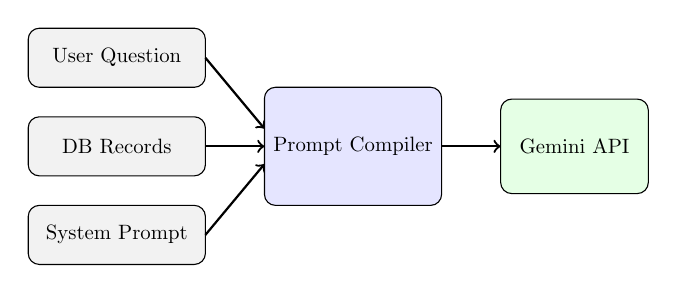
\begin{tikzpicture}[scale=0.75, every node/.style={transform shape}]
                    \draw[fill=gray!10, rounded corners] (0,3) rectangle (3,4) node[pos=.5, align=center] {User Question};
                    \draw[fill=gray!10, rounded corners] (0,1.5) rectangle (3,2.5) node[pos=.5, align=center] {DB Records};
                    \draw[fill=gray!10, rounded corners] (0,0) rectangle (3,1) node[pos=.5, align=center] {System Prompt};
                    \draw[->, thick] (3,3.5) -- (4,2.3);
                    \draw[->, thick] (3,2) -- (4,2);
                    \draw[->, thick] (3,0.5) -- (4,1.7);
                    \draw[fill=blue!10, rounded corners] (4,1) rectangle (7,3) node[pos=.5, align=center] {Prompt Compiler};
                    \draw[->, thick] (7,2) -- (8,2);
                    \draw[fill=green!10, rounded corners] (8,1.2) rectangle (10.5,2.8) node[pos=.5, align=center] {Gemini API};
                \end{tikzpicture}
            \end{center}
        \end{column}
    \end{columns}
\end{frame}


% --- Section 5: Implementation Results & Discussions ---
\section{Results \& Discussion}

\begin{frame}{Working Prototype and UI Showcase}
    \begin{columns}
        \begin{column}{0.5\textwidth}
            \begin{block}{Implemented Features}
                \begin{itemize}
                    \item Vacant Room Listings on public page.
                    \item Landlord room management with Cloudinary uploads.
                    \item Dynamic VietQR generation inside invoice modals.
                    \item Bidirectional incident reporting dashboard.
                    \item Tenant personal AI chat interface.
                \end{itemize}
            \end{block}
        \end{column}
        
        \begin{column}{0.5\textwidth}
            \begin{center}
                
\includegraphics[width=1.0\textwidth]{tenant_portal_dashboard.png}
                \vskip 0.2cm
                
\includegraphics[width=1.0\textwidth]{invoice_payment_modal.png}
            \end{center}
        \end{column}
    \end{columns}
\end{frame}

\begin{frame}{Difficulties, Limitations \& Future Work}
    \begin{columns}
        \begin{column}{0.5\textwidth}
            \begin{block}{Current Limitations}
                \begin{itemize}
                    \item \textbf{Manual Verification:} Landlords must double check their bank accounts manually.
                    \item \textbf{No Automated Tests:} Higher risk of regression during code updates.
                    \item \textbf{Dependency:} Dependent on external Google Gemini API.
                    \item \textbf{Security:} Multi-tenant isolation at application layer, not database layer.
                \end{itemize}
            \end{block}
        \end{column}
        
        \begin{column}{0.5\textwidth}
            \begin{block}{Future Directions}
                \begin{itemize}
                    \item \textbf{Payment Gateway Webhooks:} Integrate PayOS or MoMo to automatically verify bank transfers.
                    \item \textbf{Row-Level Security (RLS):} hardens multi-tenant isolation directly in PostgreSQL.
                    \item \textbf{Mobile Application:} Build React Native/Flutter portals.
                    \item \textbf{Utility History tracking.}
                \end{itemize}
            \end{block}
        \end{column}
    \end{columns}
\end{frame}

\begin{frame}{Conclusion}
    \begin{block}{Key Contributions}
        \begin{itemize}
            \item Constructed a functional SaaS prototype that digitizes small-scale rental operations.
            \item Effectively integrated AI into business rules using database context prompting.
            \item Designed a modular, clean codebase matching modern software engineering standards.
        \end{itemize}
    \end{block}
    
    \begin{center}
        \large\textbf{Thank you for listening! \\ Any questions?}
    \end{center}
\end{frame}

\end{document}
